\documentclass[12pt,aspectratio=169]{beamer}

\usetheme{metropolis}

\definecolor{mDarkBrown}{HTML}{FF5722}
\definecolor{mDarkTeal}{HTML}{263238}
\definecolor{mLightBrown}{HTML}{FF5722}

\usepackage{booktabs}
\usepackage{graphicx}
\usepackage{hyphenat}
\usepackage{multirow}
\usepackage{nicefrac}
\usepackage[normalem]{ulem}

\usepackage{pifont}
\newcommand{\cmark}{\ding{51}}
\newcommand{\xmark}{\ding{55}}

\usepackage{minted}
\usemintedstyle{tango}
\newminted[bash]{bash}{%
    autogobble,
    bgcolor=mDarkTeal!10,
    linenos
}
\newminted[py3]{python}{%
    python3,
    autogobble,
    bgcolor=mDarkTeal!10,
    linenos
}
\newminted[sql]{sql}{%
    autogobble,
    bgcolor=mDarkTeal!10,
    linenos
}

\usepackage{polyglossia}
\setdefaultlanguage[variant=british]{english}
\usepackage[english=british]{csquotes}

\defaultfontfeatures{Ligatures=TeX}
\setmainfont{Lucida Sans OT}
\setsansfont[Scale=MatchLowercase]{Lucida Sans OT}
\setmonofont[Scale=MatchLowercase]{Lucida Console DK}

\usepackage{mathspec}
\setmathsfont(Digits,Latin,Greek)[Numbers={Lining,Proportional}]{Lucida Bright Math OT}

\newcommand{\mat}[1]{\ensuremath{\mathbf{#1}}}

\newcommand{\R}{\ensuremath{\mathbb{R}}}

\newcommand{\E}[1]{\ensuremath{\mathbb{E}\!\left[ #1 \right]}}
\newcommand{\V}[1]{\ensuremath{\mathbb{V}\!\left[ #1 \right]}}
\newcommand{\Prob}[1]{\ensuremath{\Pr\!\left( #1 \right)}}
\newcommand{\Normal}[2]{\ensuremath{\mathcal{N}\!\left( #1, #2 \right)}}
\newcommand{\simiid}{\ensuremath{\overset{\text{\tiny i.i.d.}}{\sim}}}

\DeclareMathOperator{\logit}{logit}

\author{Gianluca Campanella}
\date{}



\title{Causality and study design}

\begin{document}

\maketitle

\begin{frame}{Contents}
    \tableofcontents[hideallsubsections]
\end{frame}

\section{What does `$X$ caused $Y$' mean?}

\begin{frame}{What is a cause?}
    \only<1>{%
        \begin{quote}
            `\ldots we may define a cause to be \emph{an object, followed by
             another, and where all the objects similar to the first are
             followed by objects similar to the second}. \\
             Or in other words \emph{where, \alert{if the first object had not
             been, the second never had existed}}.'
            \begin{flushright}
                \small%
                — D Hume (1748)
            \end{flushright}
        \end{quote}}
    \only<2>{%
        \begin{quote}
            `We think of a cause as \alert{something that makes a difference},
             and the difference it makes must be a \alert{difference from what
             would have happened without it}.
             Had it been absent, its effects — some of them, at least, and
             usually all — would have been absent as well.'
            \begin{flushright}
                \small%
                — D Lewis (1973), J Phil \textbf{70}(17)
            \end{flushright}
        \end{quote}}
\end{frame}

\begin{frame}{Counterfactual theory of causation}
    \vspace{1em}
    \begin{center}
        {\LARGE%
         $Y$ is present} \\[1em]
        \vfill
        {\large%
         but}
        \vfill
        {\LARGE%
         $Y$ wouldn't have been present \\[\medskipamount]
         if $X$ wasn't present}
    \end{center}
\end{frame}

\begin{frame}{Contribution, not attribution}
    \begin{itemize}
        \item We'd like to figure out the \alert{effect of $X$}, not the cause
              of $Y$
        \item $X$ is not `responsible' (i.e.\ the main or even the only reason)
              for $Y$
        \item Causes are not rivals: no point in `apportioning' outcomes
    \end{itemize}
    \vfill\pause
    \begin{columns}[t]
        \begin{column}{0.5\textwidth}
            \centering
            {\Huge\color{mLightBrown}\xmark} \\
            What is the cause of $Y$?
        \end{column}
        \begin{column}{0.5\textwidth}
            \centering
            {\Huge\color{mDarkTeal}\cmark} \\
            How much does $X$ affect $Y$?
        \end{column}
    \end{columns}
\end{frame}

\begin{frame}{Correlation is not causation}
    \begin{center}
        \large%
        A correlation is a relation between \alert{factual outcomes}, \\
        not between factual and counterfactual outcomes
    \end{center}
    \vfill\pause
    \begin{block}{Example}
        Taking cough syrup:\vspace{-1ex}
        \begin{itemize}
            \item Is \alert{positively correlated} with coughing
            \item Has a \alert{negative causal effect} on coughing (hopefully)
        \end{itemize}
    \end{block}
\end{frame}

\begin{frame}{Fundamental problem of causal inference}
    Causal effects are differences between:\vspace{-1ex}
    \begin{itemize}
        \item What happened
        \item What \alert{could have} happened (but didn't)
    \end{itemize}
    \vfill\pause
    \begin{center}
        \LARGE%
        \ldots and so cannot be measured!
    \end{center}
\end{frame}

\begin{frame}{Potential outcomes}
    \begin{columns}[t]
        \begin{column}{0.5\textwidth}
            \centering
            \[
                Y_{i}\!\left( 1 \right)
            \]
            is the outcome for unit $i$ that \\
            \alert{was observed} \\
            under some condition
        \end{column}
        \begin{column}{0.5\textwidth}
            \centering
            \[
                Y_{i}\!\left( 0 \right)
            \]
            is the outcome for unit $i$ that \\
            \alert{would have been observed} \\
            under some \emph{other} condition
        \end{column}
    \end{columns}
    \begin{center}
        (all other things being equal)
    \end{center}
    \vfill\pause
    \begin{center}
        \textbf{\alert{Causal effect} for unit $i$}\vspace{-1ex}
        \[
            Y_{i}\!\left( 1 \right) - Y_{i}\!\left( 0 \right)
        \]
    \end{center}
\end{frame}

\begin{frame}{Average causal effects}
    \begin{center}
        \large
        We cannot conclude whether $X$ caused $Y$ \\
        \alert{in any given case}, but\ldots
        \vfill\pause
        We can still figure out if $X$ causes $Y$ \alert{on average}
        \[
            \E{Y_{i}\!\left( 1 \right) - Y_{i}\!\left( 0 \right)}
            = \E{Y_{i}\!\left( 1 \right)} - \E{Y_{i}\!\left( 0 \right)}
        \]
    \end{center}
\end{frame}

\begin{frame}{Average causal effects are not transitive}
    \begin{itemize}
        \item $A$ causes $B$ and $B$ causes $C$ \alert{on average}
        \item Does it follow that $A$ causes $C$?
    \end{itemize}
    \vfill\pause
    \begin{center}
        \LARGE%
        \textbf{No!}
    \end{center}
    \begin{block}{Example}
        Imagine that\ldots\vspace{-1ex}
        \begin{itemize}
            \item $A$ causes $B$ for men only (so $A$ causes $B$ on average)
            \item $B$ causes $C$ for women only (so $B$ causes $C$ on average)
        \end{itemize}\vspace{-1ex}
        \ldots then there is no one for whom $A$ causes $C$ through $B$!
    \end{block}
\end{frame}

\section[How can we decide if \\ `$X$ caused $Y$'?]%
        {How can we decide if `$X$ caused $Y$'?}

\begin{frame}{There is no causation without manipulation\ldots}
    \begin{center}
        \large%
        \ldots because we need to be able to observe what happens under
        different conditions \alert{all other things being equal}
    \end{center}
    \vfill\pause
    \begin{center}
        \LARGE%
        Try it and find out!
    \end{center}
\end{frame}

\section{Study design}

\begin{frame}{Study designs}
    \begin{columns}[t]
        \begin{column}{0.5\textwidth}
            \begin{center}
                \textbf{Observational} \\[1em]
                The researcher observes \\
                \alert{but does not alter} \\
                what occurs
            \end{center}
        \end{column}
        \begin{column}{0.5\textwidth}
            \begin{center}
                \textbf{Experimental} \\[1em]
                The researcher \\
                \alert{intervenes to change reality}
                \\ then observes what happens
            \end{center}
        \end{column}
    \end{columns}
\end{frame}

\begin{frame}{Observational studies}
    \begin{center}
        Selection based on\ldots
    \end{center}
    \begin{columns}[t]
        \begin{column}{0.33\textwidth}
            \centering
            Exposure $X$ \\[\bigskipamount]
            $\downarrow$ \\[\bigskipamount]
            \textbf{Cohort}
        \end{column}
        \begin{column}{0.33\textwidth}
            \centering
            Outcome $Y$ \\[\bigskipamount]
            $\downarrow$ \\[\bigskipamount]
            \textbf{Case\hyp{}control}
        \end{column}
        \begin{column}{0.33\textwidth}
            \centering
            Neither \\[\bigskipamount]
            $\downarrow$ \\[\bigskipamount]
            \textbf{Cross\hyp{}sectional}
        \end{column}
    \end{columns}
\end{frame}

\begin{frame}[t]{Cohort studies}
    \begin{itemize}
        \item Selection based on exposure $X$
        \item \alert{Prospective}: exposure before outcome
        \item Usually very lengthy, leading to attrition
    \end{itemize}
    \vfill
    \begin{block}{Example}
        \begin{itemize}
            \item Select two groups:
                  \begin{enumerate}
                      \item Smokers
                      \item Non\hyp{}smokers
                  \end{enumerate}
            \item After 10 years, check who developed lung cancer
        \end{itemize}
    \end{block}
\end{frame}

\begin{frame}[t]{Case-control studies}
    \begin{itemize}
        \item Sampling based on outcome $Y$
        \item \alert{Retrospective}: outcome before exposure
        \item May be biased by imperfect recall
    \end{itemize}
    \vfill
    \begin{block}{Example}
        \begin{itemize}
            \item Select two groups:
                  \begin{enumerate}
                      \item Lung cancer patients
                      \item Cancer\hyp{}free `controls'
                  \end{enumerate}
            \item Ask them whether they've ever smoked
        \end{itemize}
    \end{block}
\end{frame}

\begin{frame}[t]{Cross-sectional}
    \begin{itemize}
        \item All data are collected \alert{at the same time}
        \item No distinction between exposure and outcome
    \end{itemize}
    \vfill
    \begin{columns}[t]
        \begin{column}{0.5\textwidth}
            \begin{center}
                \textbf{Strengths}
            \end{center}
            \begin{itemize}
                \item Often population\hyp{}based
                \item Less expensive
            \end{itemize}
        \end{column}
        \begin{column}{0.5\textwidth}
            \begin{center}
                \textbf{Weaknesses}
            \end{center}
            \begin{itemize}
                \item No direction of causality
                \item Over\hyp{}representation of cases with longer durations
            \end{itemize}
        \end{column}
    \end{columns}
\end{frame}

\begin{frame}{Confounding variables}
    \begin{itemize}
        \item \alert{Associated with both exposure and outcome}
        \item May explain correlations that have no direct causal connection
    \end{itemize}
    \vfill\pause
    \begin{columns}[c]
        \begin{column}{0.75\textwidth}
            \begin{block}{Example}
                `Grey hair causes heart disease'
            \end{block}
        \end{column}
        \begin{column}{0.25\textwidth}
            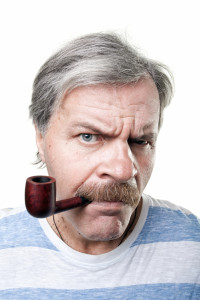
\includegraphics[height=3cm]{figures/gray_hair}
        \end{column}
    \end{columns}
\end{frame}

\begin{frame}{Experimental studies}
    \begin{center}
        Treatment randomly assigned?
    \end{center}
    \begin{columns}[t]
        \begin{column}{0.5\textwidth}
            \centering
            Yes \\[\bigskipamount]
            $\downarrow$ \\[\bigskipamount]
            \textbf{Randomised\\Controlled Trial}
        \end{column}
        \begin{column}{0.5\textwidth}
            \centering
            No \\[\bigskipamount]
            $\downarrow$ \\[\bigskipamount]
            \textbf{Quasi\hyp{}experiment} \\
            (a.k.a.\ \textbf{natural experiment})
        \end{column}
    \end{columns}
\end{frame}

\begin{frame}[t]{Randomised Controlled Trials (RCTs)}
    \begin{itemize}
        \item Control for all main forms of bias
        \item \alert{Ethical concerns}
    \end{itemize}
    \vfill
    \begin{block}{Example}
        \begin{itemize}
            \item Divide patients in two groups:
                  \begin{enumerate}
                      \item Those who take the drug
                      \item Those who take the placebo
                  \end{enumerate}
            \item Evaluate influence of drug on disease course
        \end{itemize}
    \end{block}
\end{frame}

\begin{frame}[t]{Quasi-experiments}
    \begin{itemize}
        \item More practical than RCTs
        \item \alert{Allocation bias}
    \end{itemize}
    \vfill
    \begin{block}{Example (1854 Broad Street cholera outbreak)}\vspace{-1ex}
        \begin{itemize}
            \item Public water pumps supplied by:
                  \begin{enumerate}
                      \item Southwark and Vauxhall Waterworks Company
                      \item Lambeth Waterworks Company
                  \end{enumerate}
            \item High disease rate in districts supplied by 1
            \item Water obtained downstream from sewage discharge
        \end{itemize}
    \end{block}
\end{frame}

\end{document}

